\chapter{Track Classification MVA}\label{chap:track_classification_mva}

The chapter details work on implementing a multivariate algorithm (MVA) to predict the truth origin of reconstructed tracks.
An introduction to formalisms of machine learning is given in \cref{sec:ml_background}.
In \cref{sec:track_labelling}, the truth origin label is defined, and in \cref{sec:fake_track_mva} these labels are used to train a machine learning model that can effectively discriminate between good and fake tracks.
Several studies motivated this work by demonstrating that at high \pt, \btagging performance was degraded by the presence of large numbers of poorly reconstructed or fake tracks.
If an algorithm could be trained to detect fake tracks, these could be removed before their input to the \btagging algorithms with the aim of improving performance.


\section{Machine Learning Background}\label{sec:ml_background}

Over the past few decades, machine learning (ML) techniques have become increasingly popular in high energy physics experiments due the increased volumes of high-dimensional data and improvements in the field of machine learning (in particular deep learning).
Machine learning is the process in which a computer program uses data to learn suitable parameters for a predictive model model.
This is opposed to explicitly providing instructions on how to perform a task.
A subfield known as \textit{supervised learning} is used in this work, and consists of exposing a model to a large number of labelled examples in order to extract relationships between the input data and their labels.
These relationships are often complex, and explicitly programmed rules can fail to fully capture the relationships between inputs and outputs.

%The field of machine learning aims to design computer programs which, rather than being programmed explicitly with instructions on how to perform a specific task, instead learn from a set of labelled training examples $S_i$ how to perform the task for themselves, essentially replacing the need to manually design a program to perform a specific task.
%In this section a subset of machine learning techniques called supervised learning is described.

In the simplest case, a set of $m$ labelled training examples $S = \{ (x_1, y_1) , \ldots , (x_m, y_m) \}$ is collected.
Each element $(x_i, y_i)$ consists of a input vector $x_i  \in \mathbb{R}^{\textnormal{input}}$, and the corresponding label $y_i$.
In classification problems, these labels are integer \textit{class labels} $y_i \in \{0,\ldots,N-1\}$, where $N$ is the number of classes, which specify which of a pre-determined set of categorical classes the training example belongs to.
The rest of the discussion in this chapter is limited to binary classification problems ($N = 2$).
The two classes are often referred to as signal ($y_i = 1$) and background ($y_i = 0$), which need to be separated.
Collecting sufficient and suitable data is one of the primary challenges of machine learning, as such data is not always readily available.
Fortunately, sophisticated tools to simulate particle collisions have already been developed by the scientific community \cite{leshouchesaccords, leshouchesstandardisation}. Simulation plays a key role in particle physics. More detail is given in.\todo{add section somwhere on sample info}

After obtaining suitable training data, the next step is to define a model.
Given an input domain $\mathbb{R}^{\textnormal{input}}$ and an output domain $(0, 1)$, the model
$f_\theta: \mathbb{R}^{\textnormal{input}} \to (0, 1)$ is a parameterised functional mapping from input space to output space.
Given an input example $x_i$ and a set of parameters $\theta$, the model outputs a prediction $\hat{y}_i \in (0, 1)$ for the true label $y_i$, as in
%
\begin{equation}
    f_\theta(x_i) = \hat{y}_i .
\end{equation}
%
The output $\hat{y}_i$ is in the interval $(0, 1)$ so as to be interpreted as the probability that the input example $x_i$ belongs to the signal class.
The parameters $\theta$ of the model are randomly initialised, however the model is designed to be expressive enough to correctly map the inputs $x_i$ to the outputs $y_i$ given the correct choice of parameters.
The model is then trained, which amounts to showing the model a series of labelled training examples and modifying the parameters of the model based on its performance.


\subsection{Neural Networks}\label{sec:neural_nets}

Neural networks (NNs) are a common choice for the machine learning model $f$ since they have the ability to approximate any function \cite{HORNIK1989359} and are easy to train via backpropagation \cite{rumelhart1986learning}.

\subsubsection{Artificial Neurons}

The basic functional component of a NN is the \textit{artificial neuron} or node, which is loosely inspired by a mathematical model of a biological neuron \cite{mcculloch1943logical, hopfield1987neural}.
An artificial neuron is defined by its parameters or \textit{weights} $\theta$ and a choice of activation function.
Each neuron takes a fixed number of inputs and computes the dot product of the input and weight vectors $x^T \theta$ and additionally adds a constant bias term $\theta_0$.
This term plays the role of a trainable constant value that is independent of the inputs.

\begin{figure}[!htbp]
    \centering
    \usetikzlibrary{matrix,chains,positioning,decorations.pathreplacing,arrows}
\begin{tikzpicture}[
    init/.style={
      draw,
      circle,
      inner sep=2pt,
      font=\Huge,
      join = by -latex
    },
    squa/.style={
      draw,
      inner sep=2pt,
      font=\Large,
      join = by -latex
    },
    start chain=2,node distance=13mm
    ]
    \node[on chain=2] 
      (x2) {$x_i^2$};
    \node[on chain=2,init] (sigma) 
      {$\displaystyle\Sigma$};
    \node[on chain=2,squa,label=above:{\parbox{2cm}{\centering Activation \\ function}}]   
      {$f$};
    \node[on chain=2,label=above:Output,join=by -latex] 
      {$\hat{y}$};
    \begin{scope}[start chain=1]
    \node[on chain=1] at (0,1.5cm) 
      (x1) {$x_i^1$};
    \end{scope}
    \begin{scope}[start chain=3]
    \node[on chain=3] at (0,-1.5cm) 
      (x3) {$x_i^3$};
    \end{scope}
    \node[label=above:\parbox{1.5cm}{\centering Bias \\ $\theta_0$}] at (sigma|-x1) (b) {};

    \draw[-latex] (x1) -- (sigma) node[midway,above] {$\theta_1$};
    \draw[-latex] (x2) -- (sigma) node[midway,above] {$\theta_2$};
    \draw[-latex] (x3) -- (sigma) node[midway,above] {$\theta_3$};
    \draw[o-latex] (b) -- (sigma);

    \draw[decorate,decoration={brace,mirror}] (x1.north west) -- node[left=10pt] {Inputs} (x3.south west);
\end{tikzpicture}
    \caption{
      A diagram displaying the logical flow of a single neuron with three inputs $x_i^j$.
      Each input is multiplied by a weight $\theta_j$, and the resulting values are summed.
      A bias term $\theta_0$ is added, and the result is passed to an activation function.
      Each neuron can be thought of as a logistic regression model.
    }
    \label{fig:neuron}
\end{figure}

The dot product is fed into an activation function $g$.
The activation function has several uses, most notably acting as a source of non-linearity and bounding the output of the neuron.
Some common activation functions are shown in \cref{fig:activation_functions}.
The choice of activation function can have implications for the performance and convergence of the network, since the gradient of $g$ is used to compute the weight updates during training.
This is also why input data is normalised to have zero mean and unity variance \cite{lecun2012efficient}.

\begin{figure}[!htbp]
  \centering
  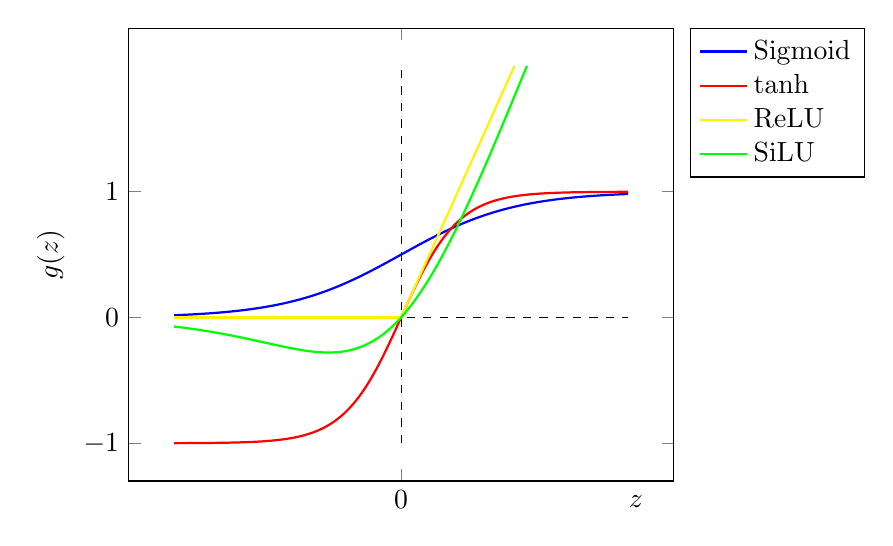
\begin{tikzpicture}
\pgfplotsset{width=8.5cm}
  \begin{axis}[
    domain=-4:4,
    xlabel=$z$,
    ylabel=$g(z)$,
    xtick={0},
    ytick={-1,0,1},
    every axis x label/.style={at={(0.9,-0.01)},anchor=north west},
    legend pos=outer north east,
    legend cell align=left
  ]
  % origin lines
  \addplot +[mark=none, black, dashed, forget plot] coordinates {(-4, 0) (4, 0)};
  \addplot +[mark=none, black, dashed, forget plot] coordinates {(0, -1) (0, 2)};

  % sigmoid 
  \addplot[thick, blue, samples=300] {1/(1+e^(-x))};%
  \addlegendentry{$\textnormal{Sigmoid}$}%

  % tanh
  \addplot[thick, red, samples=300] {tanh(x)};%
  \addlegendentry{$\textnormal{tanh}$}%
  
  % ELU
  %\addplot[thick, blue, samples=300, domain=-4:0, forget plot] {e^x - 1};%
  %\addplot[thick, blue, samples=300, domain=0:2] {x};%
  %\addlegendentry{$\textnormal{ELU}$}%

  % ReLU
  \addplot[thick, yellow, samples=300, domain=-4:0, forget plot] {0};%
  \addplot[thick, yellow, samples=300, domain=0:2] {x};%
  \addlegendentry{$\textnormal{ReLU}$}%

  % swish 
  % 1.278
  % 2.218
  \addplot[thick, green, samples=300, domain=-4:2.218] {x/(1+e^(-x))};%
  \addlegendentry{$\textnormal{SiLU}$}%

  \end{axis}%
\end{tikzpicture}
  \caption{
    Several common choices for the activation function $g$ of an artificial neuron.
  }
  \label{fig:activation_functions}
\end{figure}


\subsubsection{Networks}

Several neurons are linked together in layers to form a neural network.
The inputs are propagated layer-by-layer through the network until reaching the final output layer.
The number of layers and neurons per layer are important hyperparameters (those parameters which are not optimised as part of the training process) which influence the performance of the model.
In the case of binary classification, the final output layer consists of a single neuron with a sigmoid activation 
%
\begin{equation}\label{eq:sigmoid}
  g(z) = \frac{1}{1 + e^{-z}} ,
\end{equation}
%
which is bounded between zero and one allowing the final output to be interpreted as the probability that the input sample belongs to the signal class.
NNs have the crucial property of being differentiable functions, which facilitates training process described in the next section.

%The activation $a_i^{(l)}$ is the output of the activation function $g(z)$ of the $i^{\text{th}}$ node in layer $l$. The tensor element $\Theta_{ji}^{(l)}$ is the weight connecting the $i^{\text{th}}$ node in layer $l - 1$ to the $j^{\text{th}}$ node in layer $l$. We can compute the outputs for each neuron in a layer simultaneously using ${a}_j^{(l)} = g(\Theta_{ji}^{(l)} a_i^{(l-1)})$, where the activation function is computed element wise on the vector. Computers can perform matrix operations in parallel, making a vectorised implementation such as this more efficient than calculating each output sequentially.

%Taking an item from the dataset $S$, $(\mathbf{x}_i, {y}_i)$, the input $\mathbf{x}_i$ is propagated through the network from left to right, one layer at a time. Finally, the classification result of the network, given by the output of the final neuron $\hat{\mathrm{y}} = h(\mathbf{x}_i)$, is obtained and can be compared to the true category of the data $\mathrm{y}_i$. 



\subsection{Training with Gradient Descent}\label{sec:training_sgd}

A training algorithm is used to optimise the weights of a NN after exposure to the training data.
%The performance of the trained model depends on the amount and quality of the training data, and the efficacy of the training algorithm.
The training algorithm works minimising a loss function $L$, which quantifies the error in the model's predictions for a given input.
NNs are commonly trained using backpropagation in combination with a variant of stochastic gradient descent to iteratively update the model parameters.
In binary classification problems, the binary cross entropy given in \cref{eq:bce_loss} loss if often used.
%
\begin{equation}\label{eq:bce_loss}
  L(x_i, \theta) = y_i \ln[f_\theta(x_i)] + (1 - y_i) \ln[1 - f_\theta(x_i)]
\end{equation}
%
Since the model $f$ is differentiable, the error for each parameter $\theta_i$ can be computed by taking partial derivative of $L$ with respect to the parameter.
Updated parameters $\theta_i'$ are calculated by updating the original parameter in the direction which reduces the loss.
%
\begin{equation}\label{eq:weight_update}
  \theta_i' = \theta_i - \alpha \pd{L}{\theta_i}
\end{equation}
%
The hyperparameter $\alpha$ is known as the \textit{learning rate} and dictates the size of the step taken in the direction of the slope. 
The errors for each parameter are efficiently calculated using the backpropagation algorithm.
The process of updating weights is repeated until the weights converge the network is trained.
In practice, small batches of the input data are shown to the network at a time. For each batch the average loss is calculated and the network's weights are updated.
There are many extensions and variations of the gradient descent algorithm.
This work uses the Adam optimiser which adds momentum to the weight updates (dampening oscillations) and an adaptive per-parameter learning rate \cite{2014arXiv1412.6980K}.

\begin{comment}
The gradient descent (\cref{sec:backprop_sgd}) algorithm is used to fit the model to the data.
Using \cref{eq:bce_loss}, an error for 
From \cref{eq:bce_loss}, the error on the output node can be 
The error for the final output node is computed first.
Errors for nodes in the previous layers are computed by \textit{backpropagating} this error through the network.
The error in the output node can be computed explicitly using the loss function in \cref{eq:bce_loss}.
To find the errors for the nodes in the preceding layers $\delta^{(L-1)}_i$, we need to differentiate eq. \ref{neural cost} with respect to $z^{(L-1)}_i$.
In order to perform the differentiation, we relate $z_1^{(L)} = g(z_j^{(L-1)}) \Theta_{1j}^{(L)}$.
The result,is tantamount to propagating the output error back through the network using the weights, and multiplying at each node by the derivative of the activation function. Once the errors have been propagated through the network, the partial derivatives of $J$ can be found using the final expression in eq. \ref{backprop defs}. Lastly the weights are updated simultaneously using eq. \ref{update weights}. 

gradient descent is an example of an \textit{optimisation} algorithm that minimises the cost function $J(\theta)$ (thereby fitting the logistic regression model discussed above to some data) by selecting the optimal values of $\theta$. The algorithm works by computing the partial derivatives of $J(\theta)$ with respect to the parameters $\theta$. The parameters are then altered slightly in the direction of decreasing slope, thereby reducing the cost function.
%The partial derivative of the loss function can be calculated for every parameter $\theta_i$ in the model.

The above step must be performed simultaneously for each $\theta_j$ in $\theta$, after which a new value of $J(\theta)$ can be calculated, and the process repeated. We can compute the partial derivatives of $J$ using the derivative of the logistic function from eq. \ref{eq:bce_loss}. The results are substituted into \cref{eq:weight_update} to obtain
\end{comment}





\section{Track Truth Origin Labelling}\label{sec:track_labelling}

Crucial to supervised learning techniques are are the ground truth class labels which the machine learning model is trained to predict.
A set of track truth labels which a high degree of granularity have been implemented, and are listed in \cref{tab:truth_origins}.
%
\begin{table}[!htbp]
    \footnotesize\centering
    \setlength{\tabcolsep}{0.5em} % for the horizontal padding
    \begin{tabular}{lll}
        \toprule 
        \textbf{Truth Origin} & \textbf{Description} \\
        \hline
        Pileup  & From a \pp collision other than the primary interaction \\
        Fake    & Created from the hits of multiple particles \\
        Primary & Does not originate from any secondary decay \\
        fromB   & From the decay of a \bhadron \\
        fromBC  & From a \chadron decay which itself is from the decay of a \bhadron \\
        fromC   & From the decay of a \chadron which is not from teh decay of a \bhadron \\
        %fromTau & From the decay of a $\tau$ \\
        OtherSecondary & From other secondary interactions and decays \\
        \bottomrule
    \end{tabular}
    \caption{
      Truth origins which are used to categorise the physics process that led to the production of a track.
      Tracks are matched to charged particles using the truth-matching probability~\cite{PERF-2015-08}.
      A truth-matching probability of less than $0.5$ indicates that reconstructed track parameters are likely to be mismeasured and may not correspond to the trajectory of a single charged particle.
      The ``OtherSecondary'' origin includes tracks from photon conversions, \Kshort and $\Lambda^0$ decays, and hadronic interactions.
    }
    \label{tab:truth_origins}
\end{table}
%
For the fake track classification tool, the origins in \cref{tab:truth_origins} are used to construct a binary label by labelling all fake tracks which are not also fromB as background, and all other tracks (i.e. good tracks and fake fromB tracks) as signal.
The fake track classifier is then trained to distinguish between these two categories of tracks.
Fake tracks are defined using the \textit{truth-matching probability} (TMP), defined in \cref{eq:tmp_def}.
This is a weighted sum of the number of hits on a track which are from the same truth particle, versus the total number of hits on the track.
The weights are subdetector-dependent are designed to account for the varying number of layers in each of the subdetectors.
%
\begin{equation}\label{eq:tmp_def}
    \textnormal{TMP} = 
    \frac{
        10 N_{\textnormal{Pix}}^{\textnormal{good}} + 
        5  N_{\textnormal{SCT}}^{\textnormal{good}} + 
           N_{\textnormal{TRT}}^{\textnormal{good}}
        }{
        10 N_{\textnormal{Pix}}^{\textnormal{all}} + 
        5  N_{\textnormal{SCT}}^{\textnormal{all}} + 
            N_{\textnormal{TRT}}^{\textnormal{all}}
        }
\end{equation}
%
The labelling scheme has designed to be useful beyond the classification of good and fake tracks.


\section{Fake Track Identification Tool}\label{sec:fake_track_mva}

The rate of fake tracks increases at high transverse momentum as shown in \cref{fig:fakerate_vs} due to the difficulties in track reconstruction outlined in \cref{sec:b_track_reco_challenges}.
The performance of \btagging algorithms is reduced as a direct result of the presence of these fake tracks as shown for SV1 in \cref{fig:sv1_perf_nofake}.

To identify and remove fake tracks, a NN classification tool was trained with good tracks as the signal class and fake tracks as the background class.
Due to the imbalance between the two classes (with fake tracks being relatively uncommon), a weight was added to the loss function for the background class to account for this.
The NN was made up of two hidden layers with 100 nodes each. The ReLU activation function was used in conjunction with the Adam optimiser.

\begin{figure}[!htbp]
  \centering
  \begin{subfigure}[b]{0.48\textwidth}
      \centering
      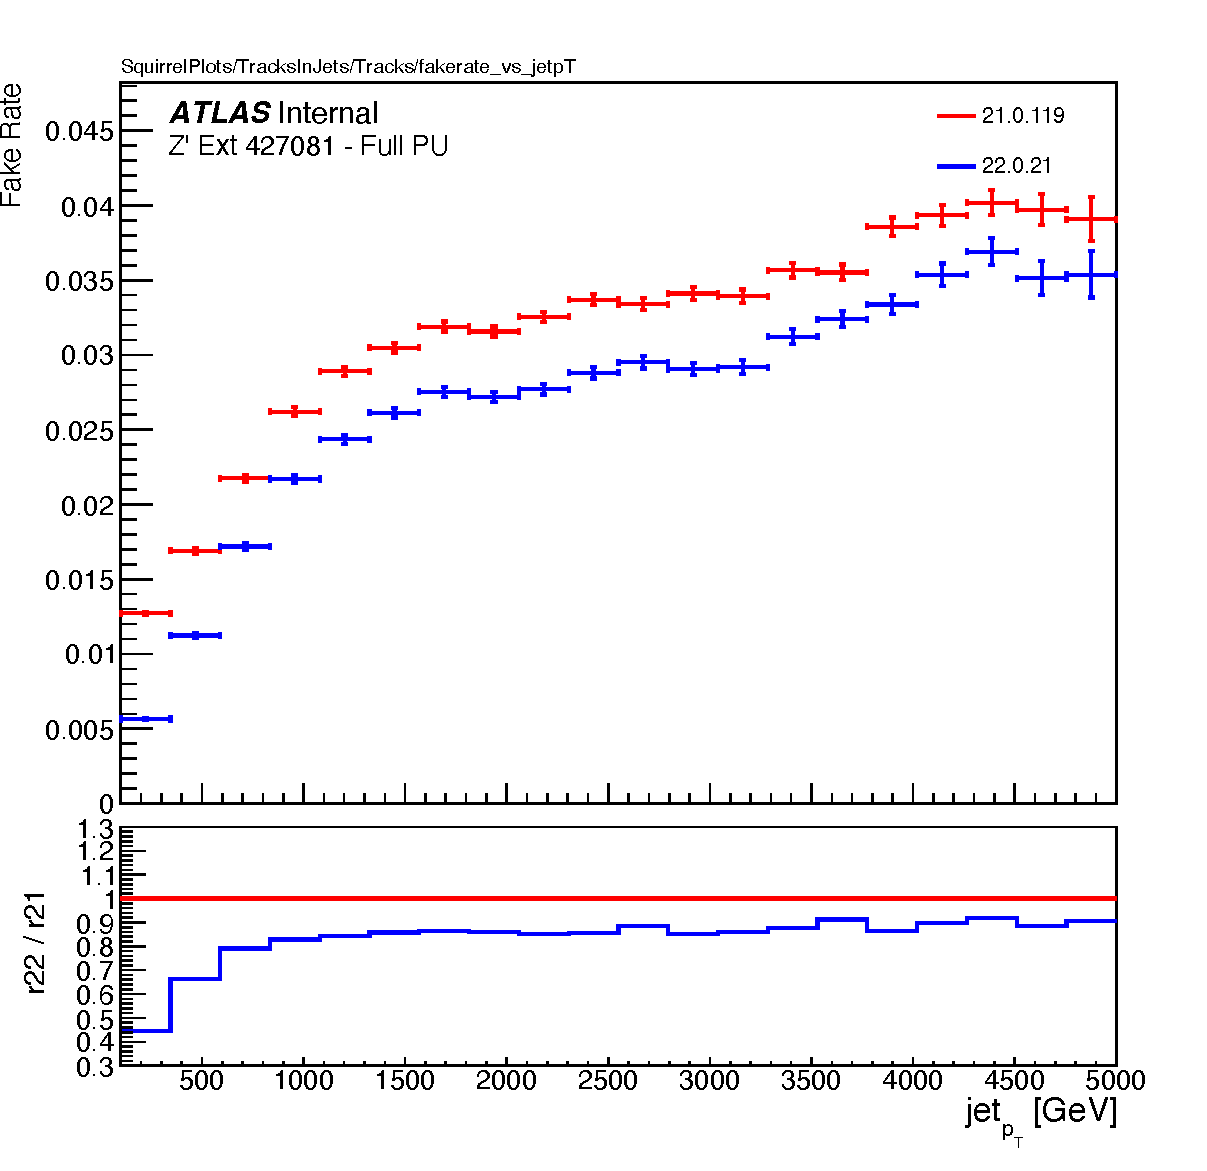
\includegraphics[width=\textwidth]{chapters/track_classifier/figs/fakerate_vs_pt.pdf}
  \end{subfigure}
  \quad
  \begin{subfigure}[b]{0.48\textwidth}
      \centering
      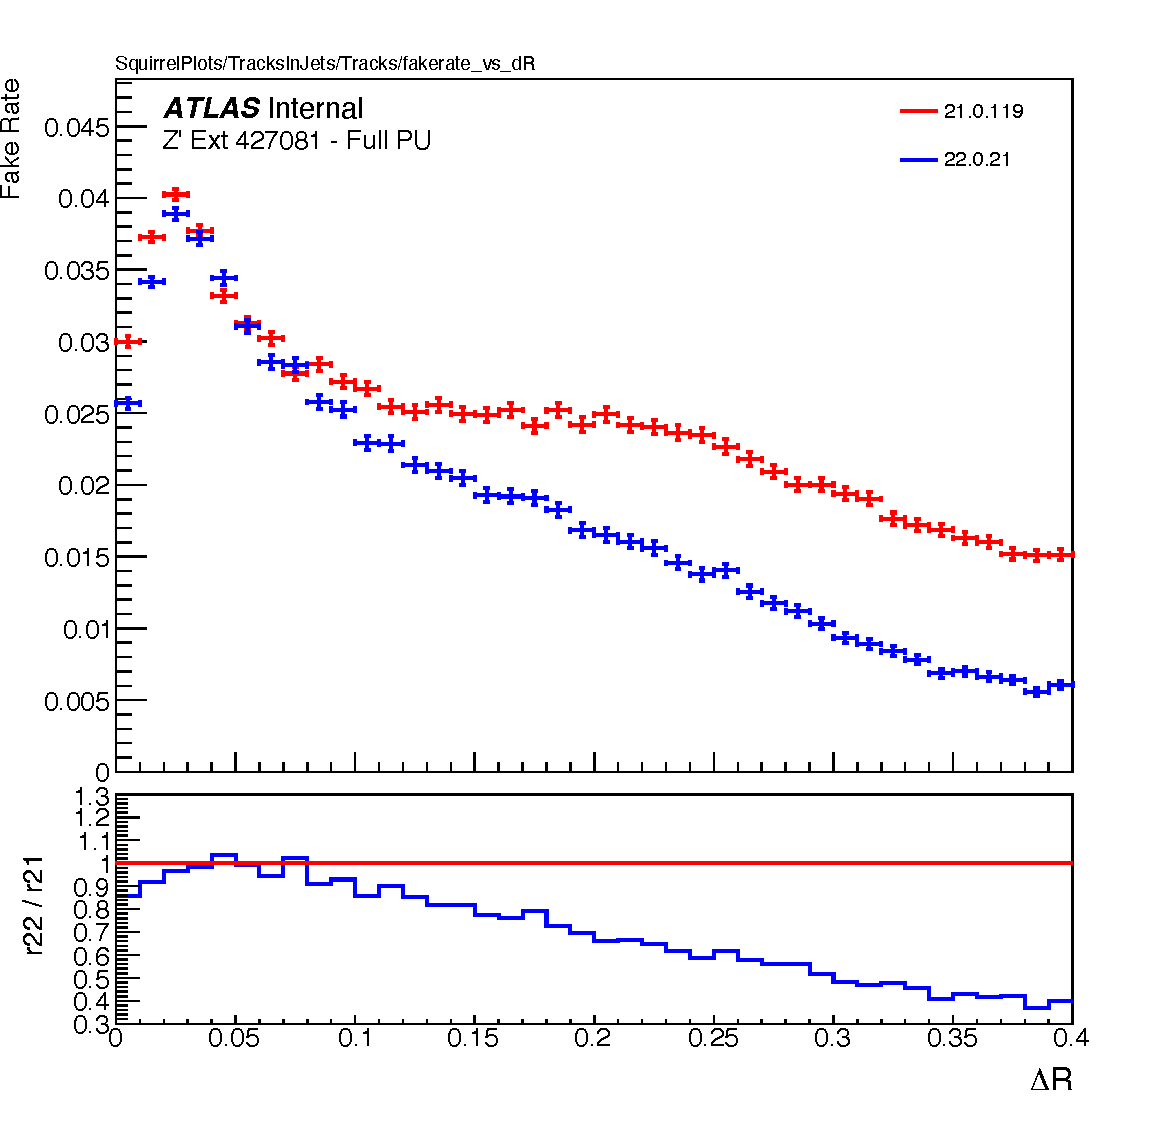
\includegraphics[width=\textwidth]{chapters/track_classifier/figs/fakerate_vs_dr.pdf}
  \end{subfigure}
  \caption{
    Rate of fake tracks as a function of jet transverse momentum (left) and $\DeltaR(\textnormal{track}, \textnormal{jet})$ (right).
    The rate of fake tracks increases significantly as a function of \pt, and also increases as the distance to the jet axis decreases, and the number of tracks in the jet increases (not shown).
  }
  \label{fig:fakerate_vs}
\end{figure}

\begin{figure}[!htbp]
    \centering
    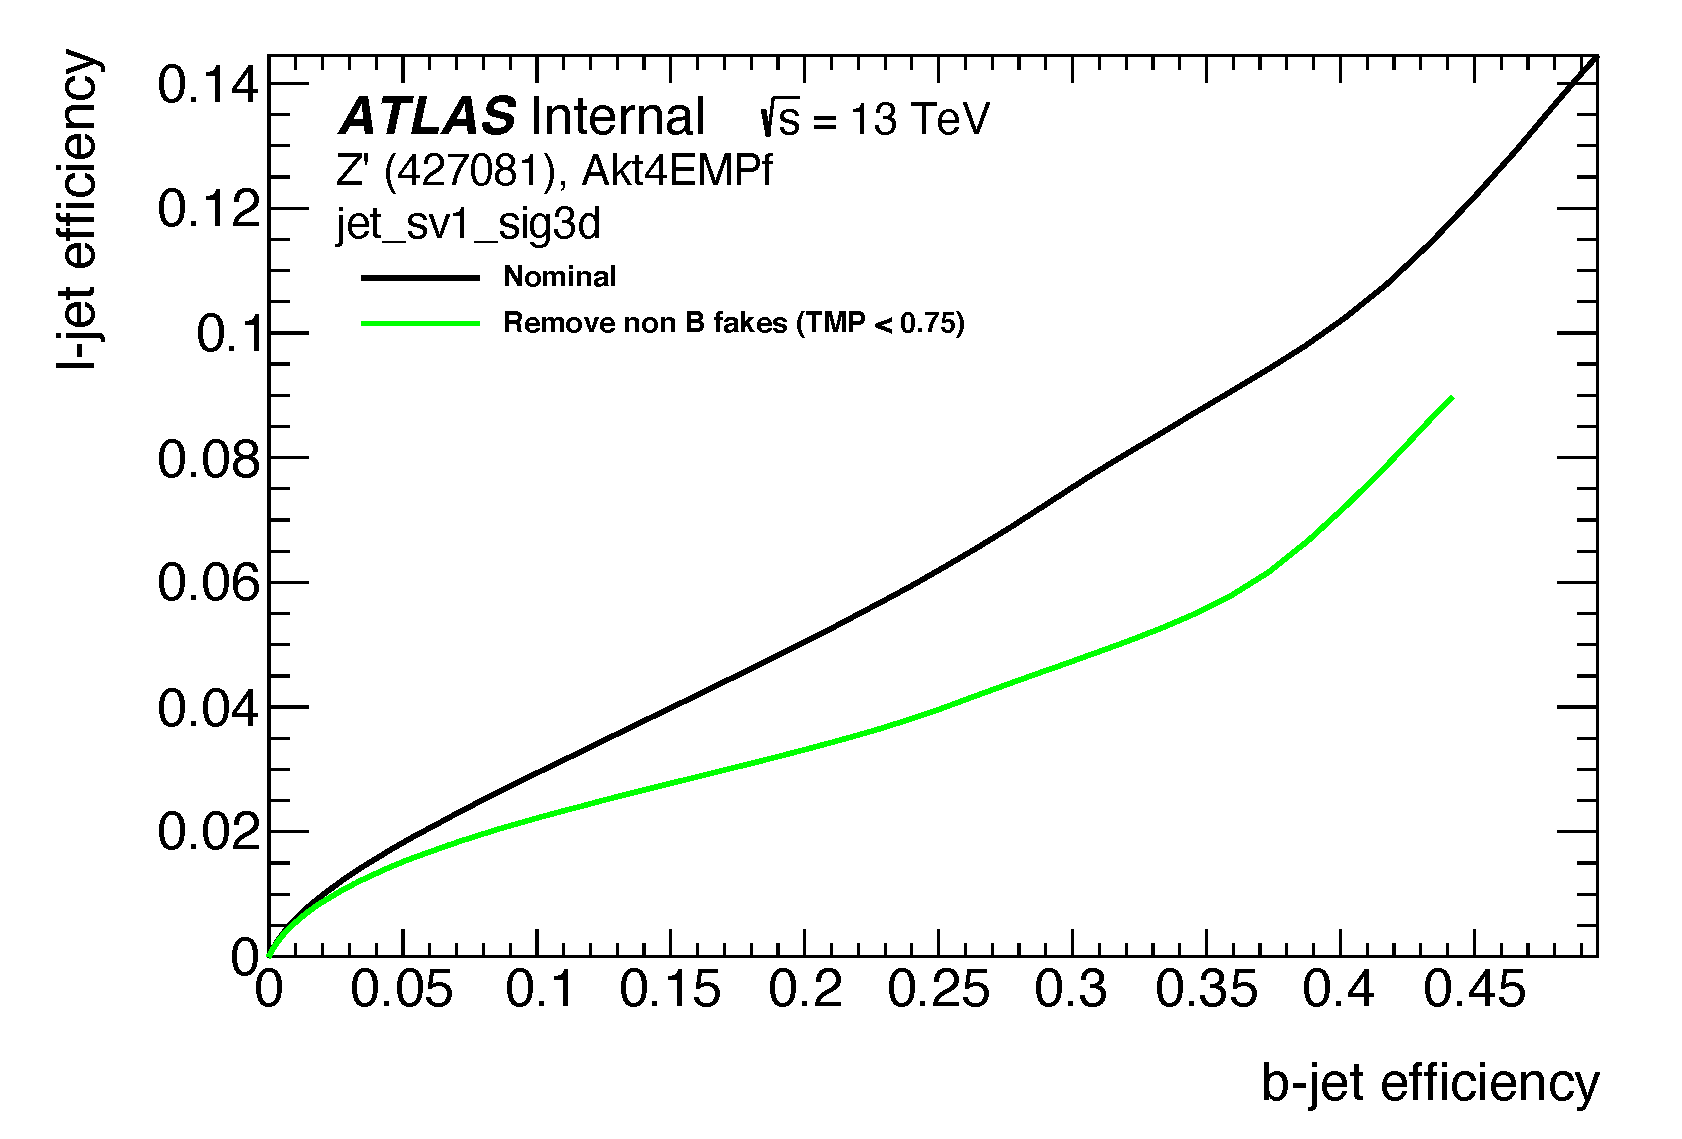
\includegraphics[width=0.7\textwidth]{chapters/track_classifier/figs/sv1_perf_nofake.pdf}
    \caption{
      The \ljet efficiency of the low level tagger SV1 as a function of \bjet efficiency for the nominal tracking setup (black) and for the case where fake tracks which are not from the decay of a \bhadron are removed.
      The \ljet efficiency is decreased, demonstrating that the presence of fake tracks is detrimental to algorithm performance.
    }
    \label{fig:sv1_perf_nofake}
\end{figure}

Inputs to the model are described in \cref{sec:fake_mva_model_inputs}, while fake track removal performance is given in \cref{sec:fake_track_mva_results}.

\subsection{Model Inputs}\label{sec:fake_mva_model_inputs}

%\newcommand{\ipdefsfootnote}{%
%Impact parameter significances are defined as the IP divided by its corresponding uncertainty, $\dzerosig = d_0 / \dzerouncert$ and $\zzerosig = z_0 / \zzerouncert$.
%Track IP significances are lifetime signed according to the track's direction with respect to the jet axis and the primary vertex \cite{PERF-2012-04}.
%}

The fake track MVA is given two jet variables and 20 tracking related variables for each track fed into the network.\todo{copied from GN1, but fake track mva uses deta instead deta dphi}
The jet transverse momentum and signed pseudorapidity constitute the jet-level inputs, with the track-level inputs listed in \cref{tab:fake_mva_track_inputs}.
Full track parameter information and associated uncertainties, along with detailed hit information, carry valuable information about the jet flavour.

\begin{table}[!htbp]
  \footnotesize\centering
  \setlength{\tabcolsep}{0.5em} % for the horizontal padding
  \begin{tabular}{ll}
    \toprule 
    \textbf{Jet Input} & \textbf{Description} \\
    \hline
    $\pt$ & Jet transverse momentum \\
    $\eta$ & Signed jet pseudorapidity \\
    \toprule
    \textbf{Track Input} & \textbf{Description} \\
    \hline
    $\pt$ & Track transverse momentum \\
    $\DeltaR$ & Angular distance between the track and jet \\
    $d_0$  & Closest distance from the track to the PV in the longitudinal plane \\
    $z_0$  & Closest distance from the track to the PV in the transverse plane \\
    nIBLHits   & Number of IBL hits \\
    nPixHits   & Number of pixel hits \\
    nSCTHits   & Number of SCT hits \\
    nTRTHits   & Number of TRT hits \\
    nBLHits    & Number of B-layer hits \\
    nIBLShared & Number of shared IBL hits \\
    nIBLSplit  & Number of split IBL hits \\
    nPixShared & Number of shared pixel hits \\
    nPixSplit  & Number of split pixel hits \\
    nSCTShared & Number of shared SCT hits \\
    nPixOutliers & Number of pixel outliers \\
    nSCTOutliers & Number of SCT outliers \\
    nTRTOutliers & Number of TRT outliers \\
    $r$      & Radius of first hit \\
    $nDOF$   & Number of degrees of freedom on the track \\
    FracRank & Ambiguity solver ordering variable \\
    \bottomrule
  \end{tabular}
  \caption{
    Input features to the \GNN model.
    Basic jet kinematics, along with information about the reconstructed track parameters and constituent hits are used.
    Shared hits, are hits used on multiple tracks which have not been classified as split by the cluster-splitting neural networks~\cite{PERF-2015-08}, while split hits are hits used on multiple tracks which have been identified as merged.
    A hole is a missing hit, where one is expected, on a layer between two other hits on a track.
    The track leptonID is an additional input to the \GNNLep model.
  }
  \label{tab:fake_mva_track_inputs}
\end{table}

Track selection follows the loose selection described in \rcite{ATL-PHYS-PUB-2020-014} and outlined in \cref{tab:fake_track_mva_selections}, which was found to improve the flavour tagging performance compared to previous tighter selections, whilst ensuring good resolution of tracks and a low fake rate \cite{PERF-2015-08}.

\begin{table}[!htbp]
  \footnotesize\centering
  \setlength{\tabcolsep}{0.5em} % for the horizontal padding
  \begin{tabular}{ll}
    \toprule 
    \textbf{Parameter} & \textbf{Selection} \\
    \hline
    $\pt$                & $> 500$ MeV \\
    $|d_0|$              & $< 3.5$ mm \\
    $|z_0 \sin\theta|$   & $< 5$ mm \\
    Silicon hits         & $\ge 8$ \\
    Shared silicon hits  & $< 2$ \\
    Silicon holes        & $< 3$ \\
    Pixel holes          & $< 2$ \\
    \bottomrule
  \end{tabular}
  \caption{
    Quality selections applied to tracks,
    where $d_0$ is the transverse IP of the track, $z_0$ is the longitudinal IP with respect to the PV and $\theta$ is the track polar angle.
    Shared hits are hits used on multiple tracks which have not been classified as split by the cluster-splitting neural networks~\cite{PERF-2015-08}.
    Shared hits on pixel layers are given a weight of 1, while shared hits in the SCT are given a weight of 0.5.
    A hole is a missing hit, where one is expected, on a layer between two other hits on a track.
    }
  \vspace{4mm}
  \label{tab:fake_track_mva_selections}
\end{table}


\begin{itemize}
  \item network structure
  \item trained on x tracks
  \item train test
  \item input variables
  \item samples -- borrow from gnn note
  \item performance plots
  \item impact on btagging
\end{itemize}

\subsection{Results}\label{sec:fake_track_mva_results}

\begin{table}[!htbp]
  \footnotesize\centering
  \setlength{\tabcolsep}{0.5em} % for the horizontal padding
  \begin{tabular}{lllll}
      \toprule
      \multirow{2}{2cm}{MVA Output Cut} & \multicolumn{2}{l}{Good Track Efficiency} & \multicolumn{2}{l}{Fake Track Efficiency} \\
      & All & FromB & All & FromB \\
      \hline
      0.06 & \pct{98.8} & \pct{98.9} & \pct{45.6} & \pct{39.8} \\
      0.12 & \pct{97.3} & \pct{97.5} & \pct{59.4} & \pct{53.6} \\
      \bottomrule
  \end{tabular}
  \caption{
    Good and fake track selection efficiencies for the combined \ttbar and \Zprime samples.
    Two working points are defined.
  }
  \label{tab:fake_track_mva_effs}
\end{table}



\section{Conclusion}\label{sec:fake_track_mva_conclusion}

Fake tracks, which are prevalent in the core of high \pt jets, are shown to have an adverse impact on \btagging performance.
A ML tool to identify fake tracks has been developed, which can be used to limit the number of fake tracks being inputted to downstream \btagging algorithms.
These fake or poorly reconstructed tracks could also be remove in other places\todo{keep?}

Another application of this tool is to isolate a relatively pure sample of fake tracks to estimate the fake track rate in data, which can be used for tracking recommendations.

A more advanced approach than detecting and removing fake tracks is to attempt to determine whether a track is good or fake, but allow any downstream tagging algorithms to use this information when coming to a descision about wether to tag a jet, rather than removing the track as an input.

The approach here works on a track-by-track basis, but a more sophisticated approach would consider the correlations between the tracks inside a jet, as shown in \cref{chap:gnn_tagger}.

Preliminary studies into a version of the tool which are used to select heavy flavour tracks from \bhadron decays have have led to the development of a mutliclassification approach...